\documentclass[10pt]{article}
\usepackage[margin=0.6in]{geometry}
\usepackage{graphicx}
\usepackage{booktabs}
\usepackage{pdfpages}
\usepackage{tikz}
\usepackage{hyperref}
\usepackage{wrapfig}
\usepackage{enumitem}
\usepackage{titlesec}
\titlespacing{\section}{0pt}{*1.5}{*1.0}
\titlespacing{\subsection}{0pt}{*1.2}{*0.8}

\clubpenalty=10000
\widowpenalty=10000
\usepackage{subcaption}
\begin{document}
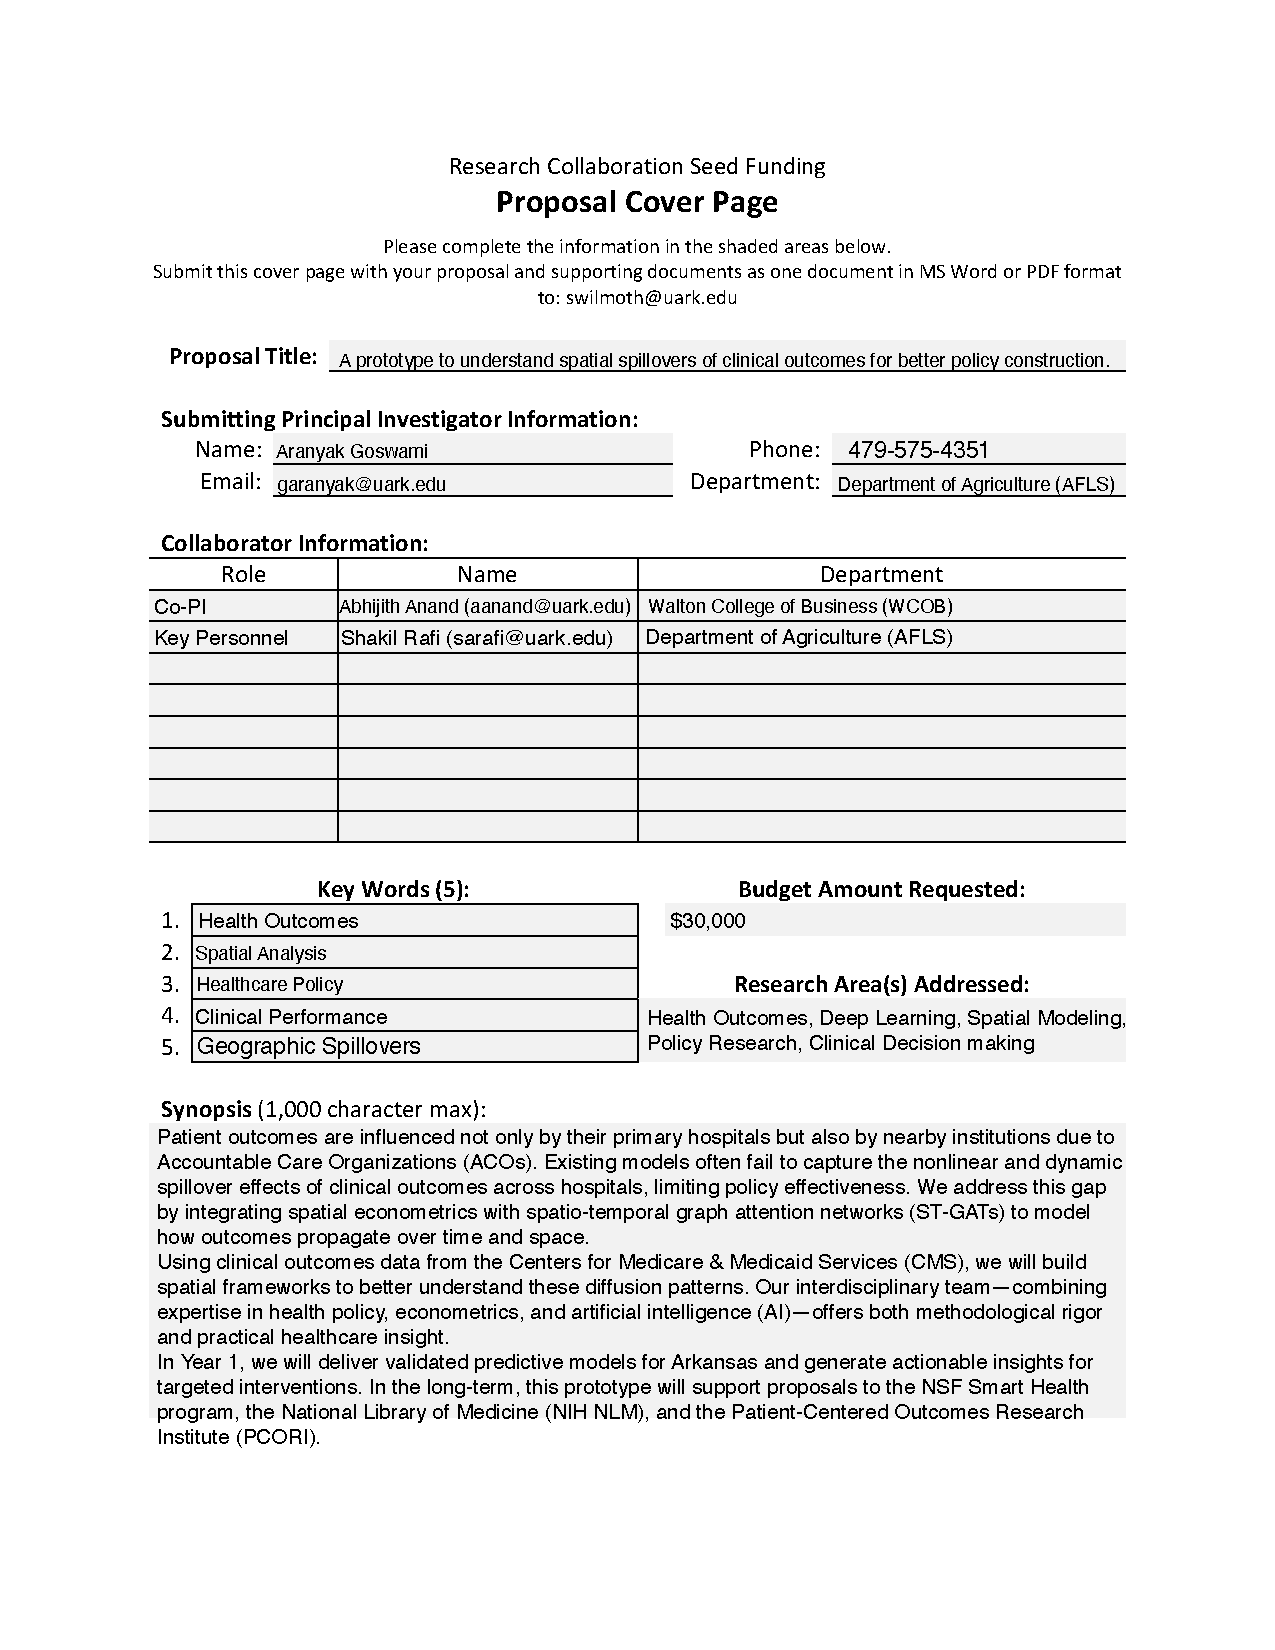
\includepdf{cover-filled.pdf}

\subsection*{Introduction}

%Due to the structure of Accountable Care Organizations (ACOs), healthcare outcomes and clinical practices are rarely confined to a single institution as they spread through the networks of hospitals with ACOs and even outside ACOs. Such spillovers are further shaped by the geographical proximities and structural hierarchies adopted by individual states and counties. This suggests that healthcare performance is not only locally determined but also influenced by broader institutional and governance ecosystems. 
%
% These spillovers unfold dynamically, driven by regulatory changes like the HITECH Act \cite{noauthor_hitech_2011}, public health crises such as the COVID-19 pandemic \cite{senathirajah_impact_2024}, and local administrative shifts \cite{di_paolo_harrison_influence_2022}. To capture this complexity, researchers have advanced models and frameworks that account for both spatial and temporal variations, including spatial panel models \cite{fischer_spatial_2010} and instrumental variable frameworks \cite{chesher_what_2013}, tools that are critical for understanding how healthcare performance propagates across interconnected systems.

Accountable Care Organizations (ACOs) (networks of clinicians, hospitals, and healthcare providers) are set up in a way such that what happens in one hospital often affects others. For example, changes in clinical practice, policy responses, or healthcare outcomes do not stay neatly within one hospital, they ``spill over'' to nearby institutions, both within the ACO and beyond. These spillover effects are shaped by geography (how close hospitals are to each other) and by the state or county-level systems that manage healthcare delivery. In other words, a hospital's performance is not determined in isolation, it is influenced by what is happening around it. These phenomena are formally known as \textit{spillover effects}.

For example, if Washington Regional Hospital drastically improved its mortality rate from childbirth, outpatient centers nearby in Northwest Arkansas would see a concomitant improvement in their childbirth mortality, as would centers nearby to those centers and hence exhibit a ripple effect throughout the Northwest Arkansas region. This is valid for any such region or hospital system in the United States, and are highly amenable to modeling. 

These spillovers evolve over time, especially in response to major events like new healthcare regulations (e.g., the HITECH Act \cite{noauthor_hitech_2011}) or crises such as the COVID-19 pandemic \cite{senathirajah_impact_2024}. To understand and quantify these ripple effects, researchers use models that track changes across both space and time, such as spatial panel models \cite{fischer_spatial_2010} and instrumental variable approaches \cite{chesher_what_2013}. These tools help reveal how performance in one part of the healthcare system can influence outcomes elsewhere, sometimes in unexpected ways.

However, a key limitation in extant studies and research is that these frameworks falls short when data is high-dimensional, irregularly spaced, or exhibit nonlinear interactions  \cite{zhou_essays_2018}.

To address this critical gap, our proposal offers two core innovation:
\begin{enumerate}[itemsep=0pt, parsep=0pt]

	\item \textit{Collecting high-resolution data}: Unlike most studies that rely on aggregated datasets, we aim to collect and organize high-fidelity data from multiple public and private sources, that offer exceptional spatial and temporal granularity, allowing for more precise modeling of hospital performance dynamics.
	\item \textit{Cutting-edge and novel modeling techniques}: In addition to classical spatial methods (e.g., spatial autocorrelation and spatial lag models), we will implement spatio-temporal graph attention networks (ST-GATs)\cite{zhang_spatial-temporal_2019} models ideally suited to our dense dataset and capable of capturing nonlinear, directional spillover effects across both space and time. These models have seen use in traffic modeling and are ideal for spatial and temporal modeling \cite{9146162} but have yet to be used in health metrics spillover, presenting a high-risk/high-reward scenario.
\end{enumerate}
This is backed by four key strengths:
\begin{enumerate}[itemsep=0pt, parsep=0pt]
	\item \textit{Interdisciplinary high-skilled team}: This project integrates expertise in econometric modeling for electronic health records (\textbf{Dr. Aranyak Goswami}), policy and management science (\textbf{Dr. Abhijith Anand}) with advanced spatial analytics knowledge (\textbf{Dr. Shakil Rafi}), offering a synergistic approach to a complex systems problem.
	\item \textit{Preliminary analyses}: Preliminary analysis reveals statistically significant spatial spillovers across facilities, highlighting the need for more advanced modeling to capture both their magnitude and underlying mechanisms.
	\item \textit{Precedent and promising follow-up}: This project is strategically designed as a launchpad for competitive external funding from major agencies that support research on spatial modeling, healthcare analytics, and decision-making systems. For instance, the NIH recently funded research employing spatiotemporal modeling to assess healthcare outcomes (e.g., Project \#1R01DK136515-01A1). The NSF Smart Health and Biomedical Research in the Era of Artificial Intelligence and Advanced Data Science (NSF 23-614) program actively supports projects integrating machine learning, health policy, and systems-level optimization. Additionally, organizations like the National Institute for Health Care Management (NIHCM) have funded applied research on geographic disparities and healthcare performance. Our work aligns with these priorities and is well-positioned to compete for follow-on funding from the National Institutes of Health NIH, National Science Foundation NSF, Patient-centered Outcomes Research Institute PCORI, and the Agency for Health Research and Quality AHRQ in subsequent stages.
	\item \textit{Potential for expanded recruitment:} Our research demands significant effort in data acquisition, wrangling, and management representing a technically intensive task well suited for graduate students and post-docs, contingent on the availability of substantial future funding
\end{enumerate}
\subsection*{Preliminary Results}

To establish proof of concept, we conducted a preliminary analysis using two representative hospital quality metrics that are reported to CMS:
\begin{enumerate}[itemsep=0pt, parsep=0pt]
	\item \texttt{COMP\_HIP\_KNEE}: the complication rate following elective primary total hip and/or total knee arthroplasty.
	\item \texttt{MORT\_30\_HF}: the 30-day mortality rate following heart failure hospitalization.
\end{enumerate}

These metrics were selected based on their clinical relevance, availability in our dataset, and their historical use in policy evaluation and hospital benchmarking. Together, they reflect both surgical outcomes and chronic care performance, offering a robust testbed for our modeling approach.

Initial spatial analysis revealed clear patterns of regional clustering and performance diffusion, particularly among outpatient centers in proximity to major hospital hubs, see Figure 1. These patterns are informed by spillover effects known in previous literature \cite{francetic_framework_2022}, \cite{baltagi_hospital_2014}, \cite{yakusheva_health_2017}. Early runs of our spatio-temporal models show promise in capturing both directionality and intensity of influence between facilities---laying a strong foundation for the expanded analysis proposed in this grant.
\begin{figure}[htbp]
  \centering
  \begin{subfigure}[b]{0.45\linewidth}
    \centering
    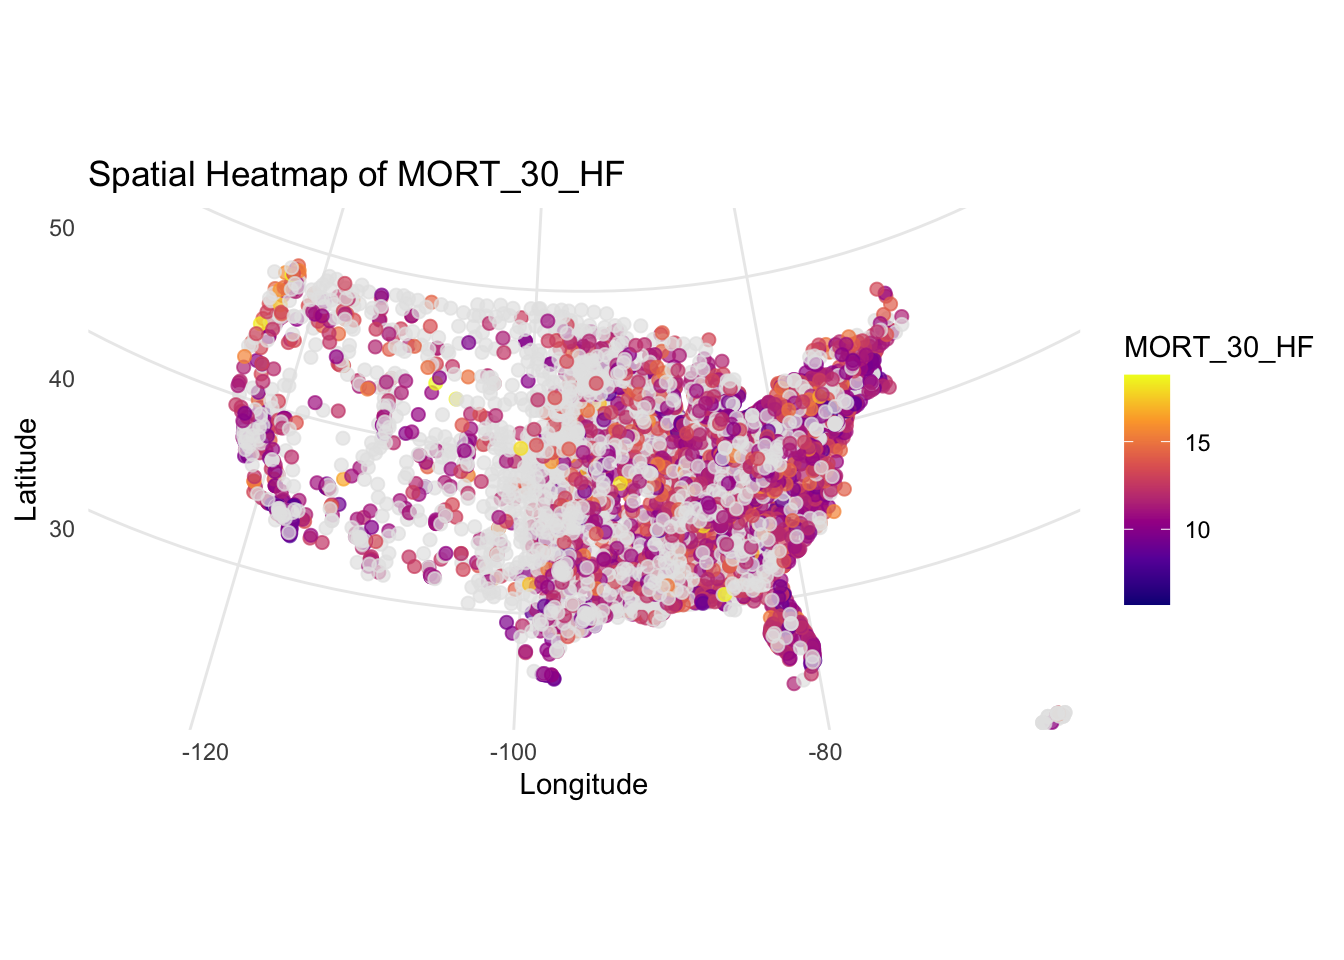
\includegraphics[width=\linewidth]{../data-folder/medicare-and-medicaid-metrics/quality-measure-2022/hospitals-10-2022/complications-and-deaths/complications-and-deaths_files/figure-html/unnamed-chunk-4-4}
    \caption{Deaths}
    \label{fig:complications}
  \end{subfigure}
  \hspace{1em}
  \begin{subfigure}[b]{0.45\linewidth}
    \centering
    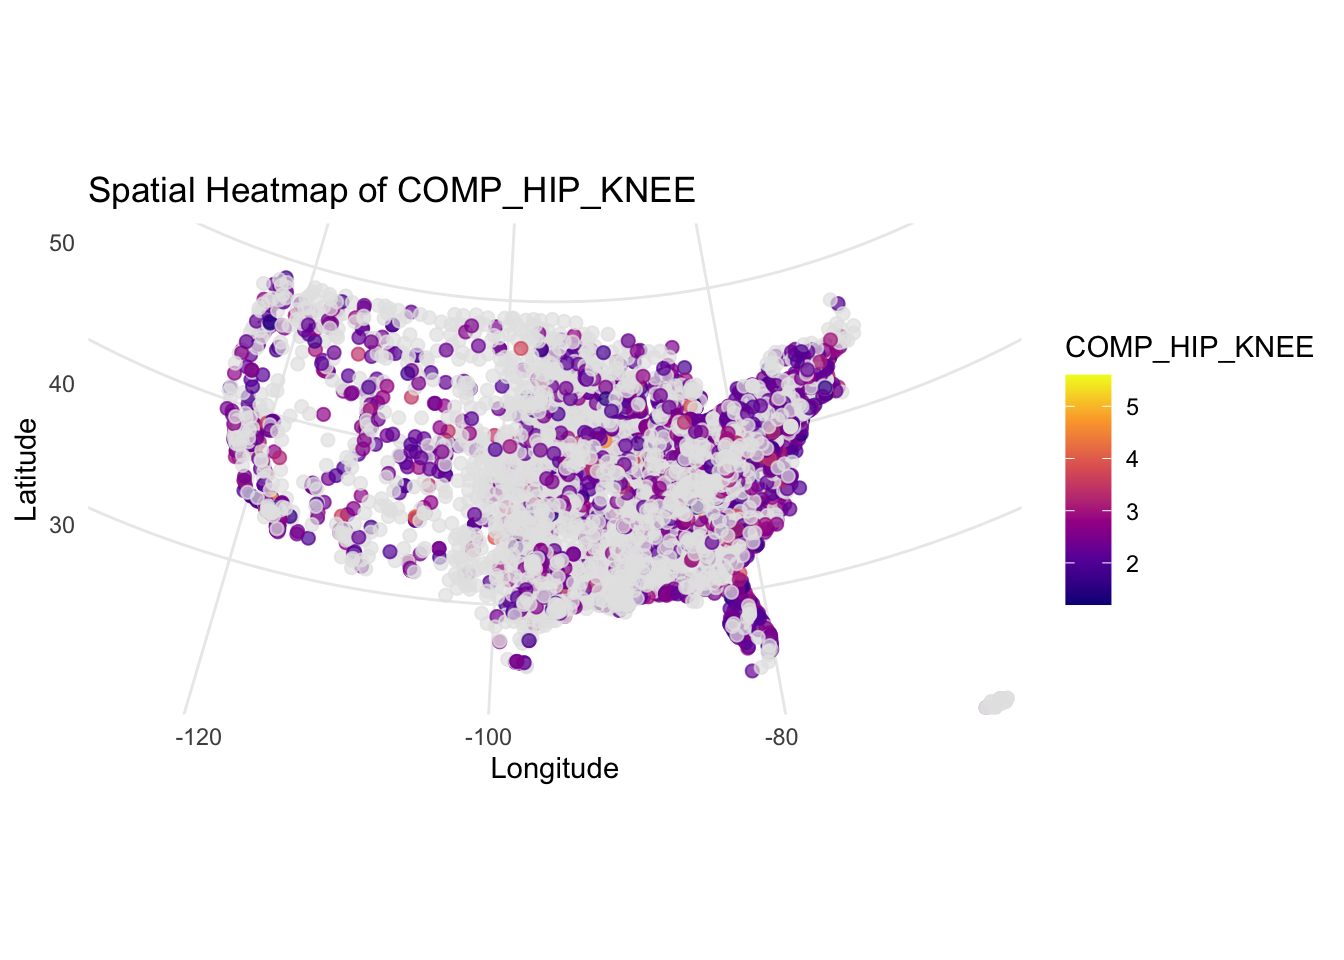
\includegraphics[width=\linewidth]{../data-folder/medicare-and-medicaid-metrics/quality-measure-2022/hospitals-10-2022/complications-and-deaths/complications-and-deaths_files/figure-html/unnamed-chunk-4-7}
    \caption{Complications}
    \label{fig:deaths}
  \end{subfigure}
  \caption{Side-by-side visualizations of deaths and complication metrics across hospitals}
  \label{fig:complications-deaths}
\end{figure}

The clustering results are backed up by spatial autoregression $\rho$ values indicating spillover effects for \texttt{MORT\_30\_HF} but not for \texttt{COMP\_HIP\_KNEE}, (see Table 1). More concretely, for every one unit increase in in \texttt{MORT\_30\_HF} at a flagship hospital there is an increase in \texttt{MORT\_30\_HF} of nearby hospitals by approximately $0.293$ with a high degree of statistical certainty.
\begin{wraptable}{r}{0.3\textwidth}
\centering
\caption{Spillover coefficient ($\rho$) for selected hospital metrics}
\begin{tabular}{@{}ll@{}}
\toprule
\textbf{Metric} & \boldmath{$\rho$} \\
\midrule
\texttt{MORT\_30\_HF} & 0.293 \\
\texttt{COMP\_HIP\_KNEE} & 0.029 \\
\bottomrule
\end{tabular}
\label{tab:spatial-autocorr}
\end{wraptable}
\indent Simulating improvements in a specific hospital metric, allows us to estimate the spillover impact of targeted interventions. This enables us to identify which hospitals act as \textit{influence hubs}, where localized improvements could lead to \textit{system-wide gains}. For example, preliminary simulations using \texttt{MORT\_30\_STK} (30-day mortality rate following stroke hospitalization) suggest that a one-unit improvement in a high-impact facility can lead to average gains of up to 0.6 units in regions like Arkansas, Alabama and southern Arizona. Please see Figure 2.

As illustrated in Figure 2, several facilities in Arkansas exhibit disproportionately high spillover scores, suggesting that targeted quality improvements in this region could yield broad regional and potentially national benefits. These results underscore the relevance of this work not just for national policy modeling, but also for state-level strategic planning in Arkansas and the broader southern U.S. healthcare system.

\begin{figure}
  \centering
  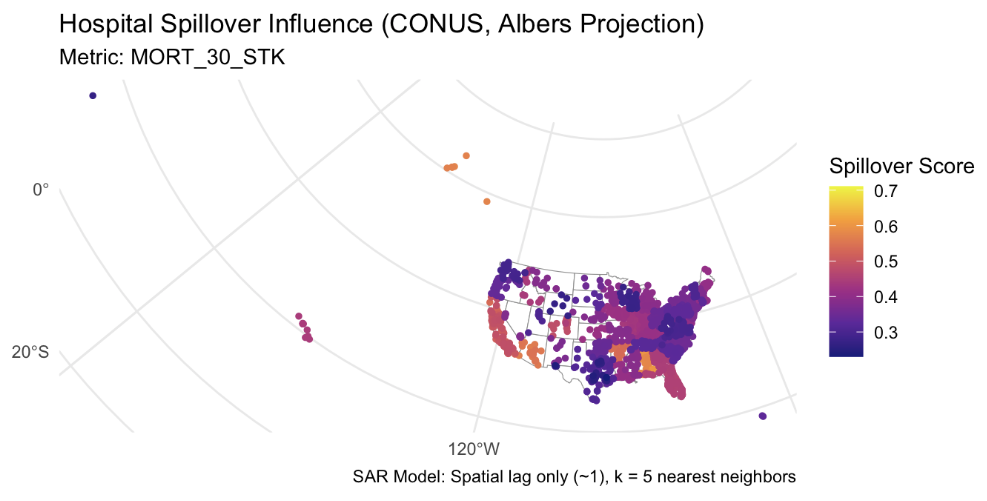
\includegraphics[scale = 0.35]{hospital-spillovers.png}
  \caption{Hospital Spillover effects showing strong spillover in Arkansas, Alabama, and southern Arizona.}
  \label{fig:wrap}
\end{figure}


\subsection*{The Proposed Method}

We will begin by collecting and integrating data from public and proprietary sources, primarily from CMS. This will require significant preprocessing and validation and is expected to take approximately one month, led by the Ph.D. student.

With our robust dataset, we will begin by estimating spatial lag models across all 143 available hospital quality metrics to quantify the direction and magnitude of spatial dependencies. Each model requires the inversion of a $4085\times 4085$ spatial weight matrix demanding significant computational resources and careful tuning for stability and interpretability.

We will then implement a spatio-temporal graph attention network (ST-GAT), initially focusing on healthcare facilities within the state of Arkansas before scaling to a nationwide model. The ST-GAT architecture is specifically designed to capture nonlinear relationships across both space and time and has been successfully applied in domains such as traffic flow forecasting and urban mobility modeling \cite{10.1145/3511808.3557705}. To the best of our knowledge this has yet to be applied to model health outcomes spillover effects, presenting a high-risk/high-reward scenario.

After initial implementation, we will iteratively refine and train our models, validating their performance against classical spatio-temporal econometric models to establish robust benchmarks.

This pipeline represents a substantial technical undertaking, well-suited to the scope of a Master's thesis or PhD dissertation and offers valuable training opportunities in applied machine learning, network science, and spatial econometrics.



\subsection*{Outcomes and Actionable Deliverables}

We propose to have the following timeline for our deliverables.

\begin{itemize}[itemsep=0pt, parsep=0pt]
\item \textbf{Month 1---2}: Data acquisition and preprocessing.
\item \textbf{Month 3---4}: Spatial lag model estimation across selected hospital metrics. 
\item \textbf{Month 5---7}: Development and training of ST-GAT models for Arkansas facilities. 
\item \textbf{Month 8---9}: Nationwide model scaling and benchmarking against traditional methods. 
\item \textbf{Month 10---11}: Analysis of influence hubs and policy simulations. 
\item \textbf{Month 12}: Drafting manuscripts, submitting grant applications, and preparing the final report.
\end{itemize}

We intend to present our preliminary findings at the 2026 Joint Statistical Meetings (JSM), scheduled for August 2026 in Boston, Massachusetts. To meet this goal, we will prepare and submit a poster abstract by the December 2025 submission deadline. Concurrently, we aim to make a preprint of our analysis publicly available on \texttt{arXiv} by Spring 2026, accompanied by open-source code and data repositories hosted on GitHub to promote transparency and reproducibility. For final publications, we will target high-impact peer-reviewed journals such as \textit{Health Economics}, and \textit{Econometrica}.

\subsection*{Budget Justification}

This budget strategically supports the successful execution and dissemination of the proposed research over a 12-month period. Part of a Ph.D. student's salary will be supported at \$1,800 per month for three months, providing critical expertise in data modeling, machine learning implementation, and manuscript development. Travel costs (\$4,000) will support attendance at a domestic conference to present findings and foster collaborations. Materials and supplies (\$7,500) cover data storage and collaboration tools necessary for secure handling and version control of high-resolution healthcare datasets.

Publication fees (\$1,602) are allocated for two open-access journal articles to ensure broad visibility and rapid dissemination of results. Other direct costs (\$6,500) are designated for cloud-based GPU access (e.g., AWS/GCP credits) and essential licensed software (e.g., MATLAB toolboxes, GraphML add-ons) required for implementing advanced spatio-temporal models. No institutional overhead is requested, ensuring that the entire budget directly supports research, dissemination, and project infrastructure.

\subsection*{Conclusion}

This project delivers a novel, interdisciplinary framework to model how healthcare outcomes propagate through institutional networks over time and space. By integrating high-resolution hospital data with cutting-edge spatiotemporal machine learning, we address a major gap in understanding systemic performance spillovers, a challenge central to health systems optimization.

Preliminary results reveal strong influence patterns and identify high-impact facilities in Arkansas where localized improvements may yield broader regional gains. These findings have immediate relevance for hospital operations, health policy, and strategic planning across disciplines.

In one year, we will produce validated predictive models, identify actionable intervention hubs, and publicly share open-source tools, preprints, and publications. These outputs represent a strong foundation for proof-of-concept success and future external funding.
The project exemplifies the type of high-risk/high-reward, cross-college collaboration this seed grant seeks to support. It brings together expertise from business, engineering, health data science and with clear alignment to external programs like NSF Smart Health, NIH, NLM, and PCORI, this initiative positions the University of Arkansas for leadership in scalable, data-driven healthcare research.

\newpage
\bibliographystyle{plain}
\bibliography{references}

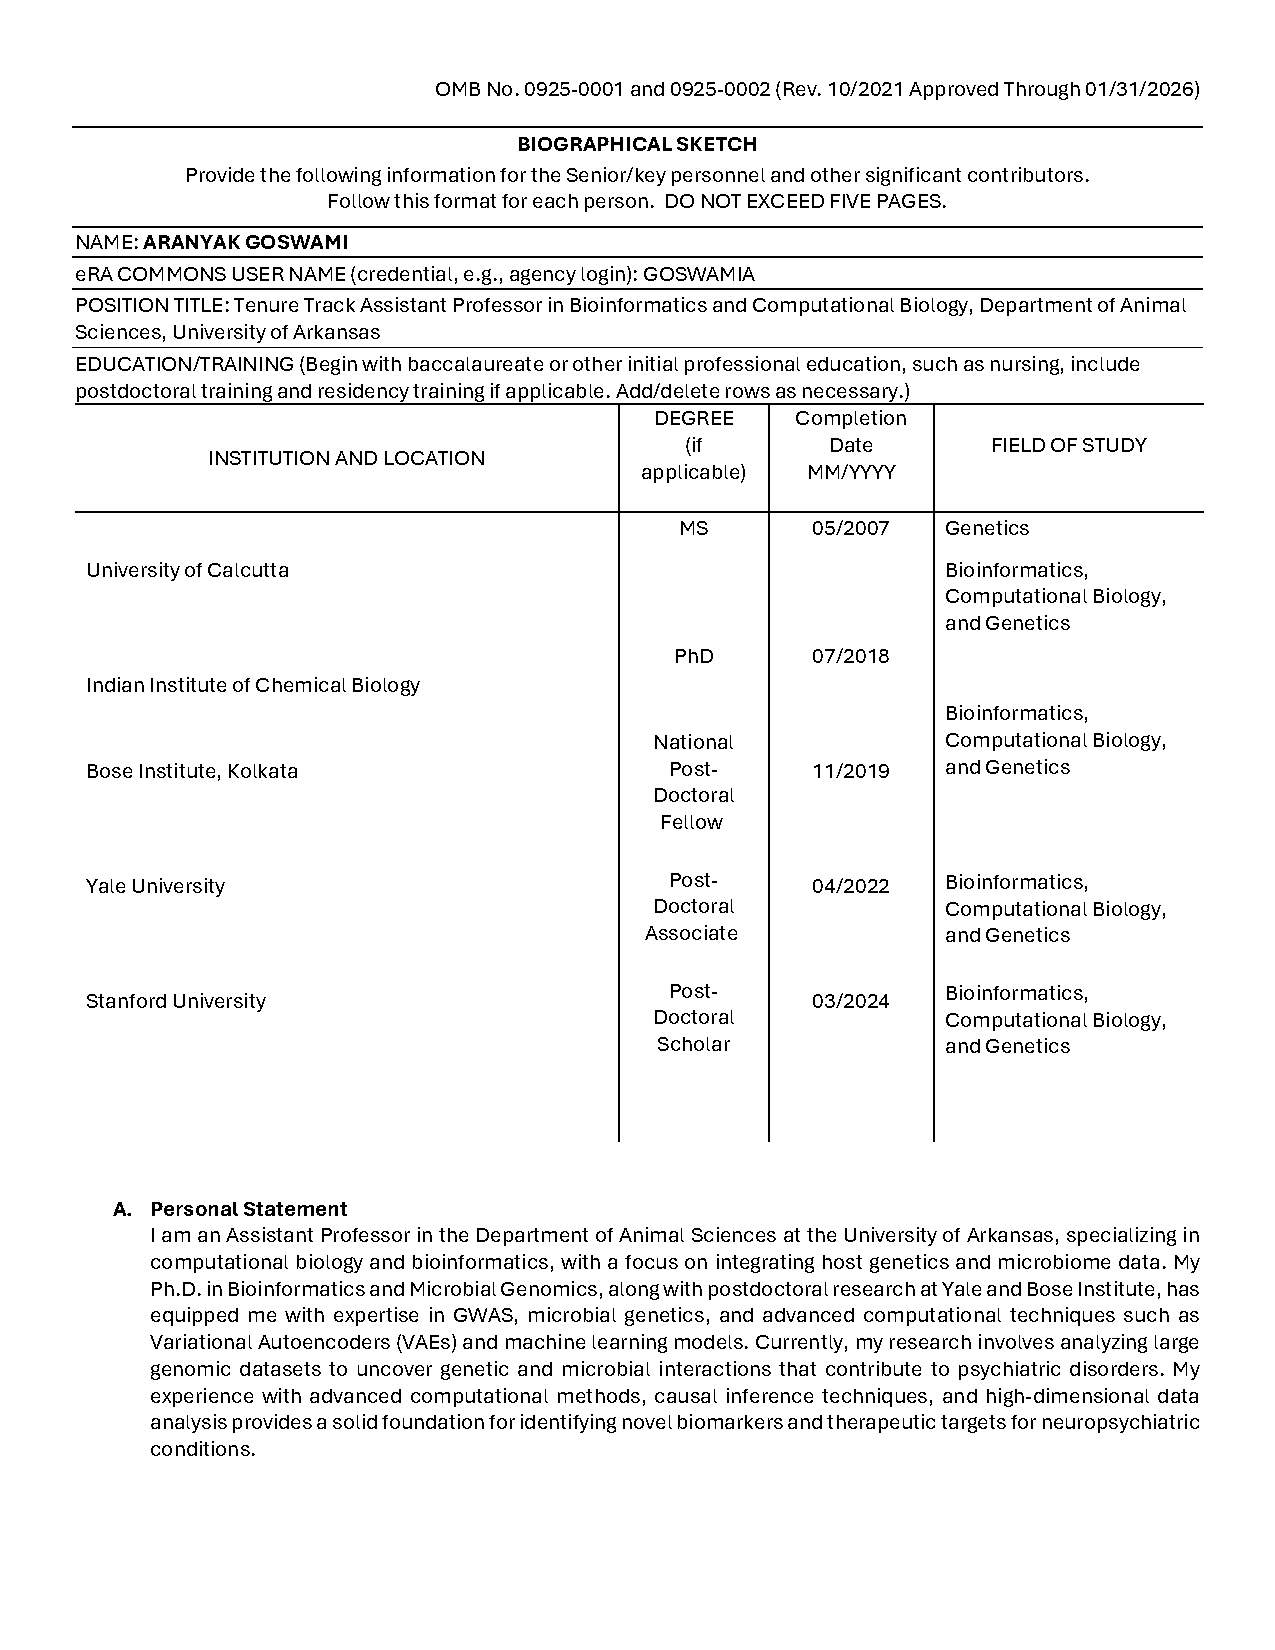
\includepdf[pages=-]{goswami-biosketch.pdf}
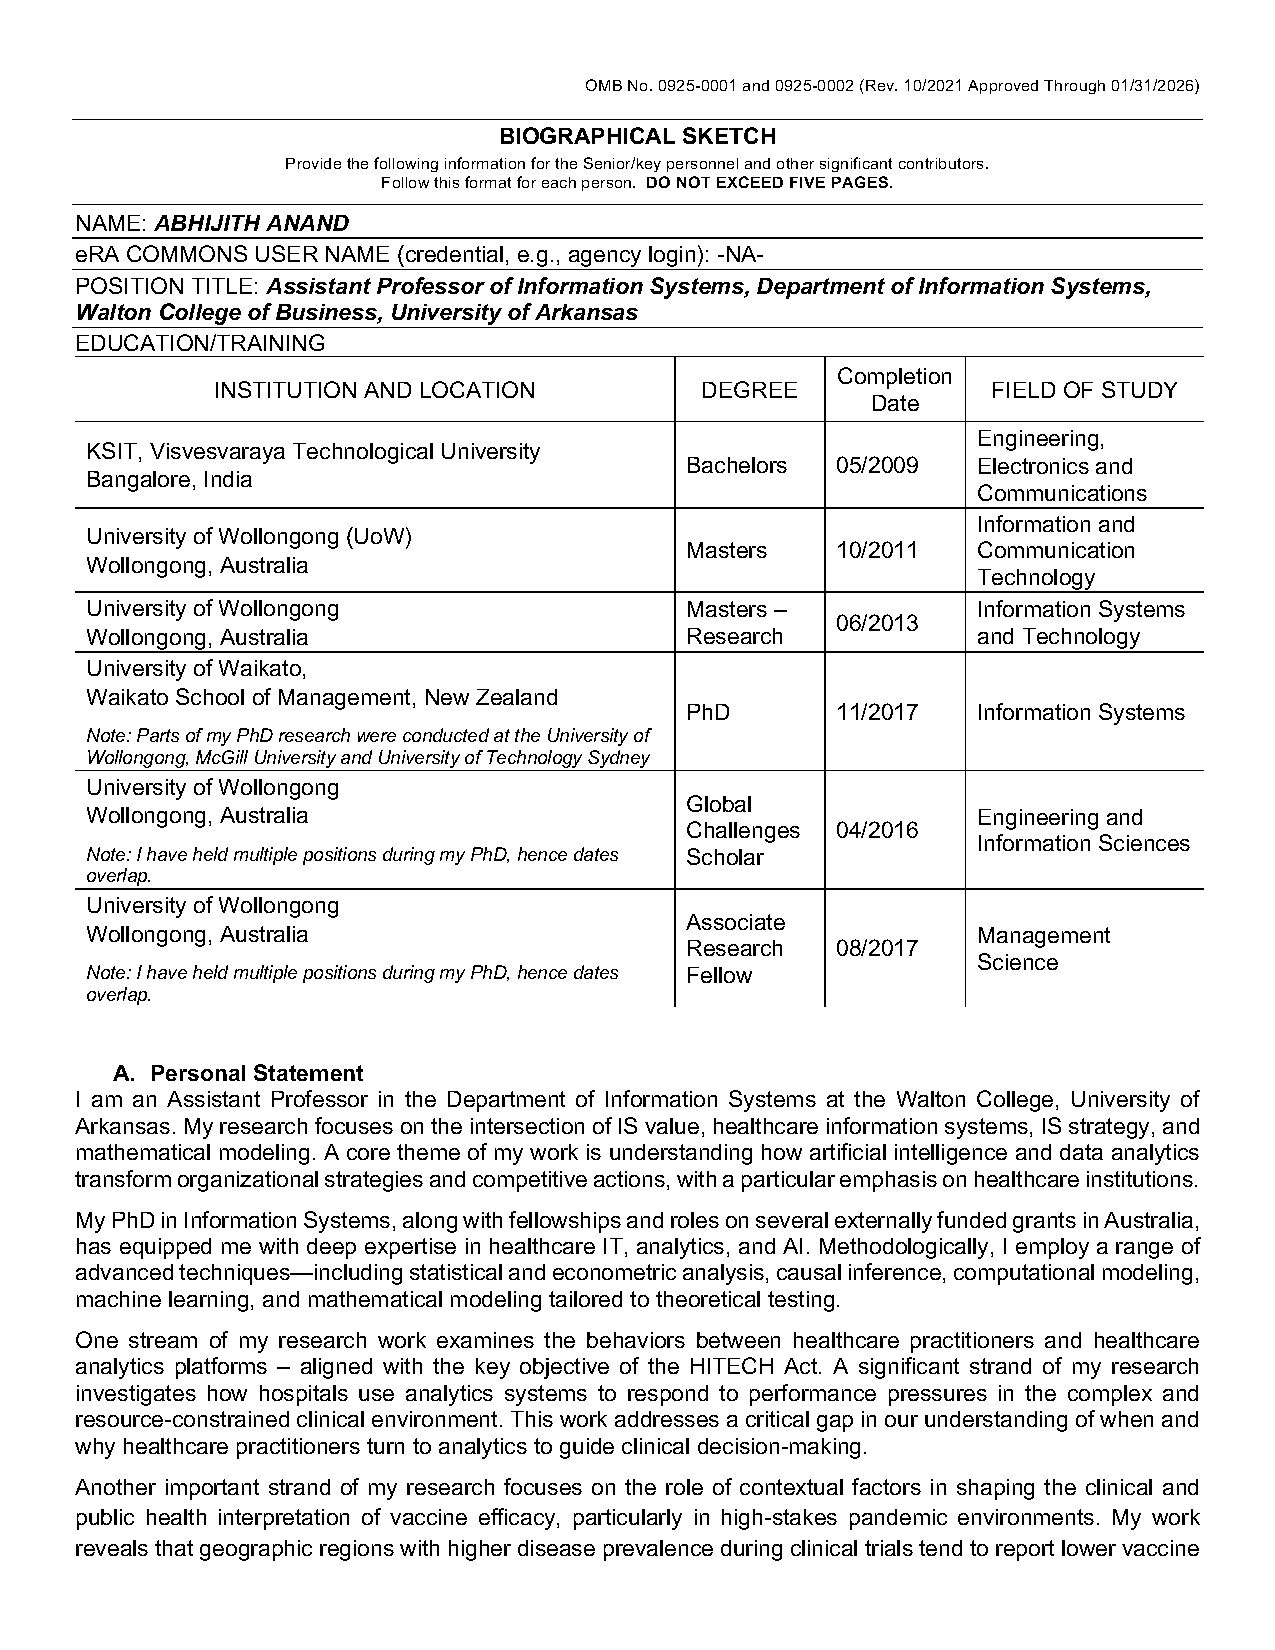
\includepdf[pages=-]{anand-biosketch.pdf}

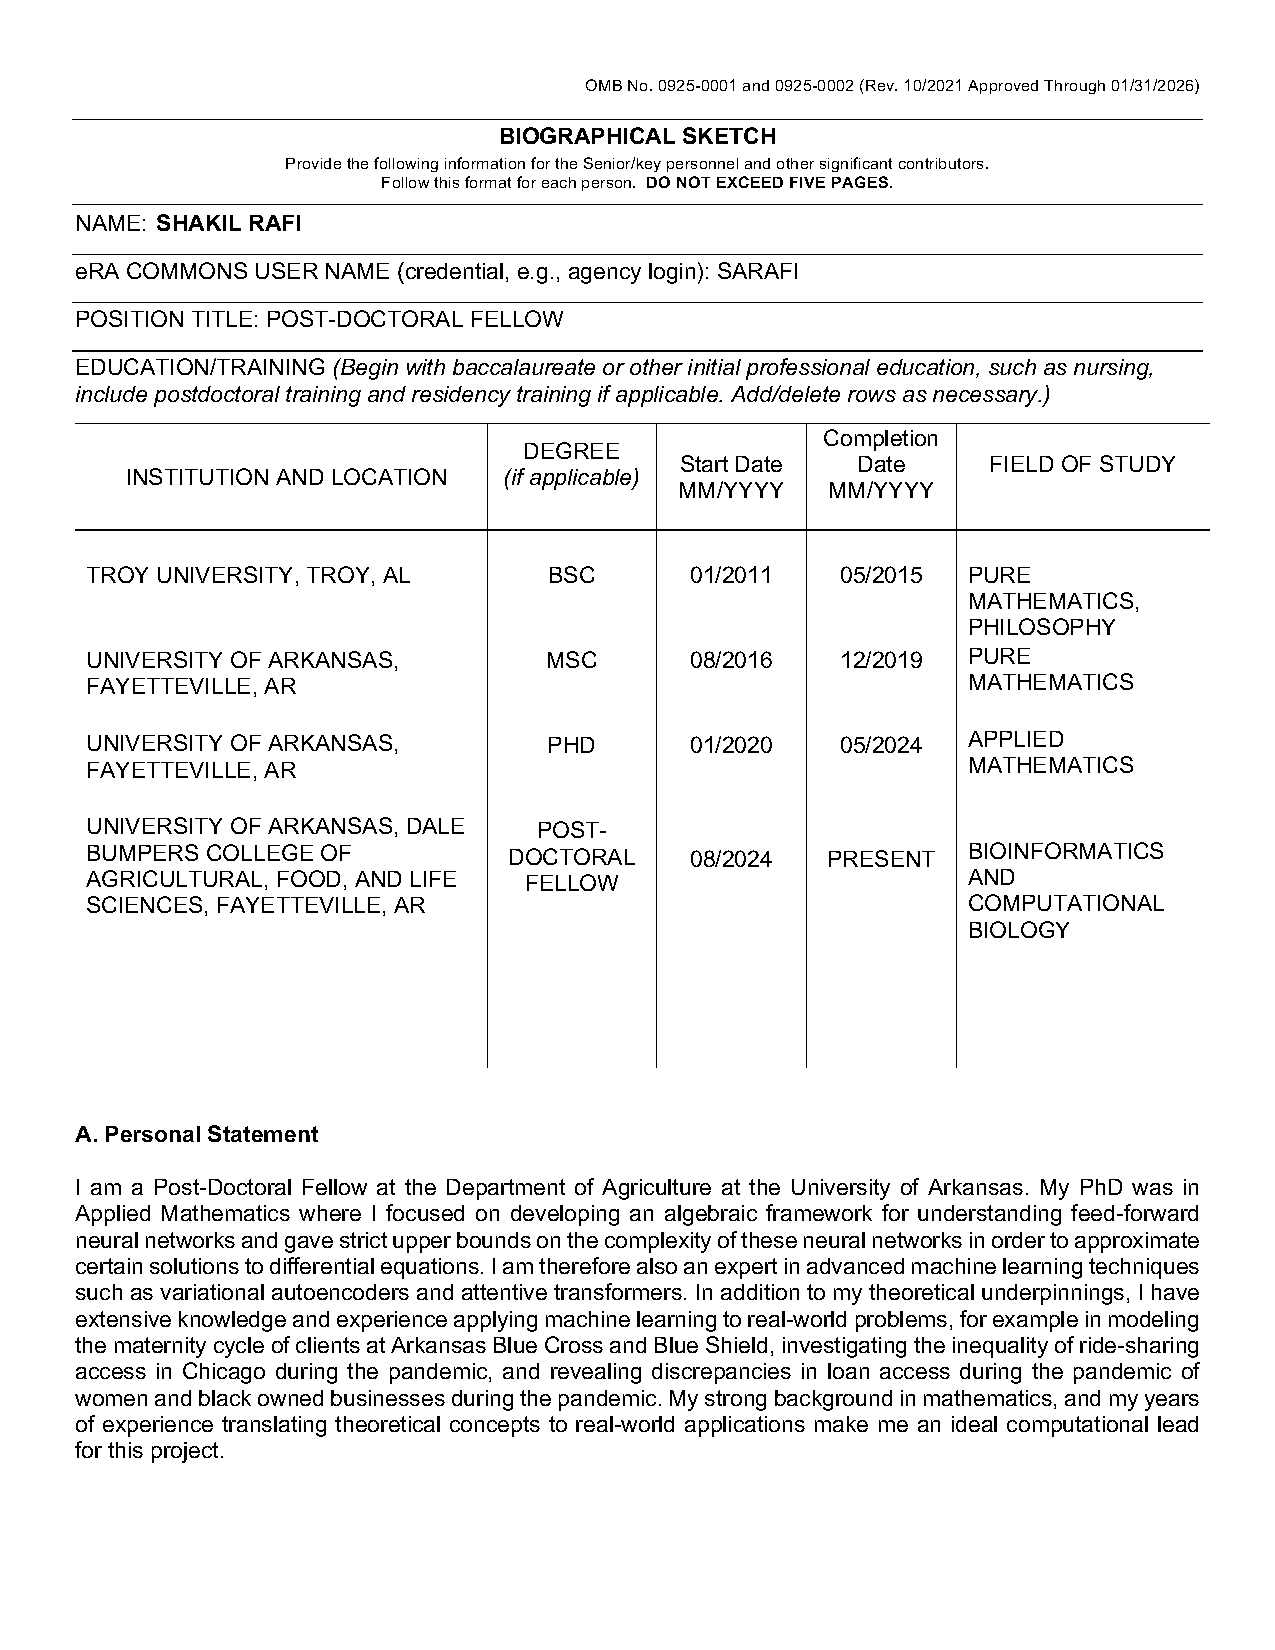
\includepdf[pages=-]{rafi-biosketch.pdf}
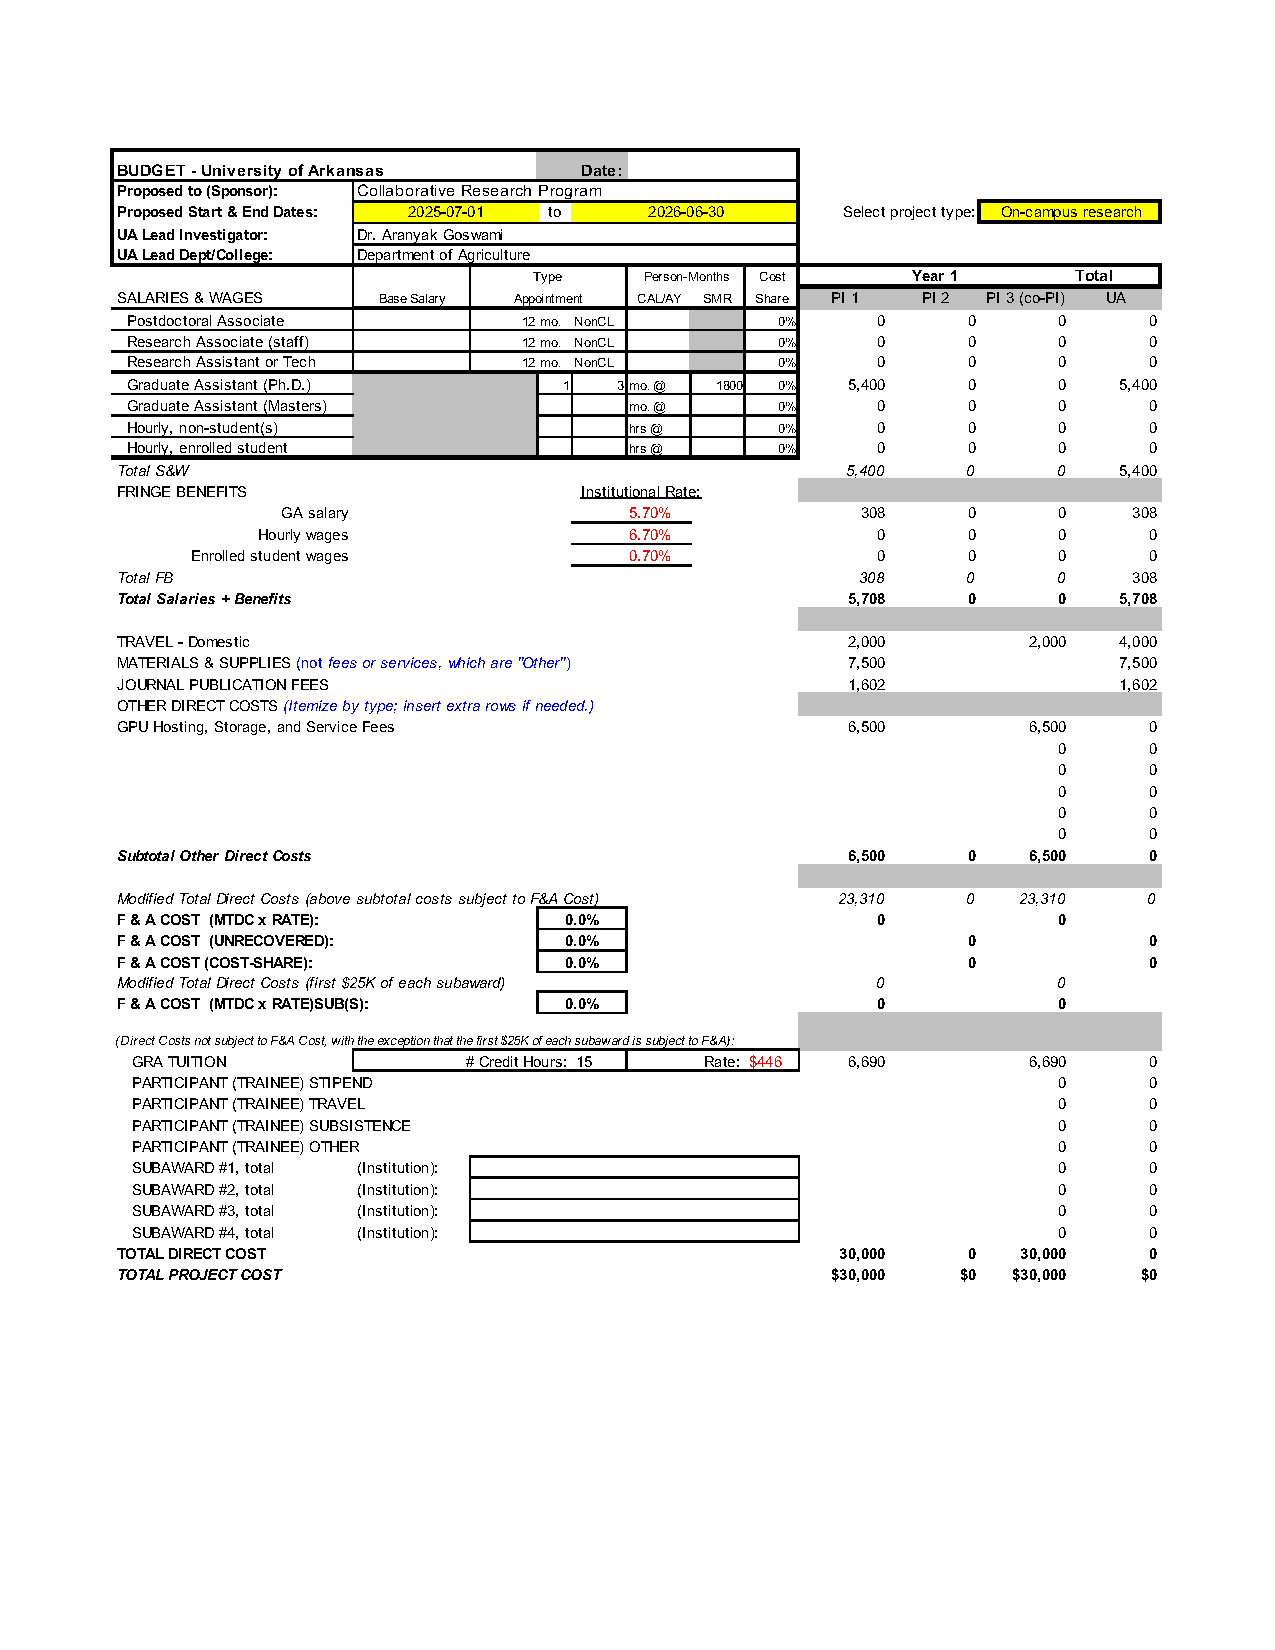
\includepdf[pages=-]{budget-template.pdf}

\end{document}